\begin{figure}[H]
    \centering
    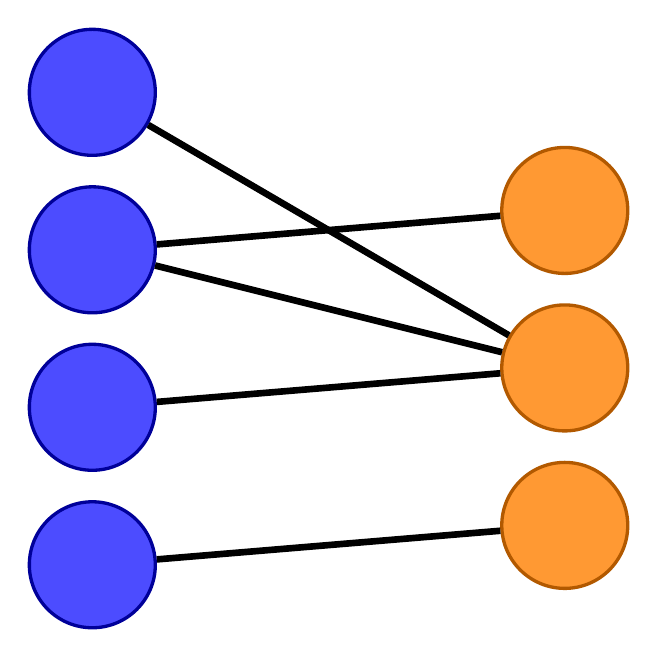
\begin{tikzpicture}[
        vertexA/.style={circle, draw=blue!60!black, fill=blue!70, very thick, minimum size=16mm},
        vertexB/.style={circle, draw=orange!70!black, fill=orange!80, very thick, minimum size=16mm},
        edge/.style={black, line width=2.4pt}
    ]
        % Conjunto A (izquierda)
        \node[vertexA] (a1) at (0,6) {};
        \node[vertexA] (a2) at (0,4) {};
        \node[vertexA] (a3) at (0,2) {};
        \node[vertexA] (a4) at (0,0) {};

        % Conjunto B (derecha)
        \node[vertexB] (b1) at (6,4.5) {};
        \node[vertexB] (b2) at (6,2.5) {};
        \node[vertexB] (b3) at (6,0.5) {};

        % Aristas (aprox. como en la imagen)

        \draw[edge] (a1) -- (b2);
        \draw[edge] (a2) -- (b1);
        \draw[edge] (a2) -- (b2);
        \draw[edge] (a3) -- (b2);
        \draw[edge] (a4) -- (b3);
    \end{tikzpicture}
    \caption{Ejemplo de grafo bipartito.}
    \label{fig:grafo-bipartito}
\end{figure}
